\documentclass[10pt,twocolumn]{article}
\usepackage[margin=0.72in,columnsep=0.24in]{geometry}
\usepackage{amsmath,amssymb,booktabs,graphicx,microtype,xcolor,hyperref,enumitem}
\hypersetup{colorlinks=true,linkcolor=blue!55!black,citecolor=blue!55!black,urlcolor=blue!55!black}
\setlist{nosep,leftmargin=*}
\setlength{\belowcaptionskip}{4pt}
\graphicspath{{figures/}}
\newcommand{\OperatingCells}{144}
\newcommand{\PracticalTies}{103}
\newcommand{\ReadoutWinners}{18}
\newcommand{\ZNEWinners}{14}
\newcommand{\InconclusiveCells}{9}
\newcommand{\HoldoutCells}{29}
\newcommand{\HoldoutCompatibility}{41.4\%}
\newcommand{\HoldoutMeanRegret}{0.0207}
\newcommand{\HoldoutMedianRegret}{0.000397}
\newcommand{\ShiftCompatibility}{50.0\%}
\newcommand{\ShiftMeanRegret}{0.00771}
\newcommand{\ShiftMedianRegret}{0}
\newcommand{\HardwareFailures}{99}
\newcommand{\NegativeGains}{179}
\newcommand{\SummaryRows}{432}
\newcommand{\ZNEValidityCells}{16}
\newcommand{\ZNECredibleCells}{5}
\newcommand{\ZNERejectedCells}{11}
\newcommand{\ZNEProbabilityRepeats}{800}
\newcommand{\ZNEUnstableRepeats}{197}
\newcommand{\ZNEDestroyedRepeats}{5}
\newcommand{\ZNEHardwareCells}{8}
\newcommand{\ZNEHardwareCredibleCells}{0}

\newcommand{\VTwoPracticalTies}{26}
\newcommand{\VTwoRawWinners}{77}
\newcommand{\VTwoReadoutWinners}{18}
\newcommand{\VTwoZNEWinners}{14}
\newcommand{\VTwoInconclusive}{9}
\newcommand{\RawWinsAccuracy}{40}
\newcommand{\RawWinsCostOnly}{37}
\newcommand{\RawWinsLowSignal}{63}
\newcommand{\HoldoutCompatibilityVTwo}{41.4\%}
\newcommand{\HoldoutStrictVTwo}{31.0\%}
\newcommand{\ShiftCompatibilityVTwo}{50.0\%}
\newcommand{\ShiftStrictVTwo}{47.2\%}
\newcommand{\HoldoutRegretMean}{0.0210}
\newcommand{\HoldoutRegretMedian}{0.0004}
\newcommand{\HoldoutRegretMax}{0.2555}
\newcommand{\ShiftRegretMean}{0.0081}
\newcommand{\HoldoutAlwaysRaw}{0.0219}
\newcommand{\HoldoutAlwaysReadout}{0.0077}
\newcommand{\ShiftAlwaysRaw}{0.0051}
\newcommand{\ShiftAlwaysReadout}{0.0101}
\newcommand{\SelectorCatastrophic}{17}
\newcommand{\SelectorCatastrophicGHZ}{8}
\newcommand{\SelectorCatastrophicLowSignal}{9}
\newcommand{\SelectorAbstentions}{6}
\newcommand{\SelectorUnnecessaryAbstentions}{5}
\newcommand{\SelectorHarm}{59}
\newcommand{\AlwaysRawHarm}{42}
\newcommand{\StrongSignalCells}{84}
\newcommand{\StrongHarmSelector}{28}
\newcommand{\StrongHarmRaw}{42}
\newcommand{\StrongHarmReadout}{19}
\newcommand{\SequentialRows}{198{,}000}
\newcommand{\NullWilsonMin}{1.7\%}
\newcommand{\NullWilsonMax}{2.7\%}
\newcommand{\NullNaiveMin}{22.4\%}
\newcommand{\NullNaiveMax}{24.9\%}
\newcommand{\NearTieShareMin}{98.1\%}
\newcommand{\NearTieShareMax}{99.8\%}
\newcommand{\NearTieUnresolvedMin}{96.0\%}
\newcommand{\NearTieUnresolvedMax}{99.7\%}
\newcommand{\BiasedRawWrong}{100\%}
\newcommand{\BiasedRawShots}{2{,}022}
\newcommand{\BiasedZNEWrong}{77\%}
\newcommand{\LifetimeRows}{60{,}480}
\newcommand{\NeverAbrupt}{0.386}
\newcommand{\NeverAsymmetric}{0.331}
\newcommand{\NeverSlow}{0.170}
\newcommand{\NeverRandom}{0.047}
\newcommand{\TriggerShotSaving}{40\%}
\newcommand{\VTwoCells}{120}
\newcommand{\VTwoDecidedCells}{26}
\newcommand{\VTwoNoSafeCells}{94}
\newcommand{\VTwoReliableCells}{14}
\newcommand{\VTwoHOneRate}{53.8\%}
\newcommand{\VTwoHOneLow}{35.5\%}
\newcommand{\VTwoAvoidedCells}{27}
\newcommand{\VTwoHTwoRate}{28.7\%}
\newcommand{\VTwoHTwoLow}{20.6\%}
\newcommand{\VTwoRegretSelector}{0.0059}
\newcommand{\VTwoRegretRaw}{0.0606}
\newcommand{\VTwoRegretReadout}{0.0033}
\newcommand{\VTwoCatastrophicSelector}{0}
\newcommand{\VTwoCatastrophicRaw}{10}
\newcommand{\VTwoCatastrophicReadout}{0}
\newcommand{\VTwoReadoutDecisionShare}{22\%}
\newcommand{\VTwoRequestShare}{50\%}
\newcommand{\VTwoUnresolvedShare}{26\%}

\newcommand{\HardwareGoMet}{1}
\newcommand{\HardwareGoTotal}{7}
\newcommand{\HardwareTriggers}{6}
\newcommand{\HardwareTriggerTotal}{6}
\newcommand{\HardwareTotalShots}{72.1}
\newcommand{\HardwareNearTieShots}{205{,}218}

% Generated by src/generate_paper_v2_assets.py from committed processed results.
\newcommand{\BandContrast}{0.611}
\newcommand{\BandContrastHigh}{0.674}
\newcommand{\BandContrastLow}{0.545}
\newcommand{\BlockedCombined}{5}
\newcommand{\BlockedRaw}{13}
\newcommand{\BlockedReadout}{7}
\newcommand{\BlockedZne}{11}
\newcommand{\BothLayersCertified}{0.502}
\newcommand{\BothLayersFalse}{0.0074}
\newcommand{\BoundaryFitBetter}{63.5\%}
\newcommand{\CertWrongNearTie}{35.9\%}
\newcommand{\CertWrongOverrotation}{6.9\%}
\newcommand{\CheckWarnShare}{76.2\%}
\newcommand{\ConditionWarnShare}{0.0\%}
\newcommand{\ConfirmClose}{12}
\newcommand{\ConfirmResolved}{13}
\newcommand{\ConfirmUnderpowered}{9}
\newcommand{\ConfirmatoryCount}{34}
\newcommand{\CorePValue}{0.001}
\newcommand{\CorePairs}{398}
\newcommand{\CoreRawError}{0.271}
\newcommand{\CoreZneError}{0.379}
\newcommand{\FullFailHigh}{100.0\%}
\newcommand{\FullFailLow}{93.0\%}
\newcommand{\FullQualityShareHigh}{98.5\%}
\newcommand{\FullQualityShareLow}{80.0\%}
\newcommand{\GateVOneFullFA}{0.018}
\newcommand{\GateVOneFullFR}{0.454}
\newcommand{\GateVOneRuntimeFA}{0.520}
\newcommand{\GateVOneRuntimeFR}{0.284}
\newcommand{\GateVTwoFA}{0.176}
\newcommand{\GateVTwoFR}{0.000}
\newcommand{\HoldoutClose}{34}
\newcommand{\HoldoutComparisons}{72}
\newcommand{\HoldoutResolved}{35}
\newcommand{\HoldoutUnderpowered}{3}
\newcommand{\LayerOneCertified}{0.518}
\newcommand{\NaiveCertified}{0.700}
\newcommand{\NaiveFalse}{0.0175}
\newcommand{\NearZeroRawBetter}{95.1\%}
\newcommand{\RawThreeRegret}{0.0024}
\newcommand{\ReachedCombined}{34}
\newcommand{\ReachedRaw}{26}
\newcommand{\ReachedReadout}{33}
\newcommand{\ReachedZne}{27}
\newcommand{\ReadoutThreeRegret}{0.0031}
\newcommand{\ReliabilityCells}{40}
\newcommand{\ThreeCostRatioSelector}{1.63}
\newcommand{\ThreeCoverageSelector}{0.64}
\newcommand{\ThreeRegretSelector}{0.0031}
\newcommand{\ThresholdNearZeroTwenty}{0.0\%}
\newcommand{\ThresholdRawTen}{46}
\newcommand{\ThresholdRawTwenty}{12}
\newcommand{\ThresholdReadoutHigh}{19}
\newcommand{\ThresholdReadoutLow}{18}
\newcommand{\ThresholdTieTen}{62}

\newcommand{\paragraphlead}[1]{\textbf{#1}\quad}
\title{When Does Quantum Error Mitigation Pay Off Under a Fixed Shot Budget?\\
Accounting, Decision Reliability, and Operational Boundaries in Simulation}
\author{Zhen-Jun Liu}
\date{November 9, 2026}

\begin{document}
\maketitle

\begin{abstract}
Quantum error mitigation (QEM) removes bias at the price of extra circuit executions and
amplified sampling variance. Whether that trade is worth making depends on what the estimate is
used for. We study unmitigated estimation, readout correction, zero-noise extrapolation (ZNE), and
their combination in noisy classical simulation, charging every calibration circuit, folded
execution, pilot, and diagnostic to one declared shot budget. The paper makes three contributions.
\emph{(i) Fixed-budget benchmarking.} On a 144-cell grid, a cost-aware oracle labels
\VTwoRawWinners{} cells as raw wins and only \VTwoReadoutWinners{} and \VTwoZNEWinners{} as readout
and ZNE wins. On 126 independent circuits frozen by noiseless value, ZNE beats raw more often at
large references than near zero, by \BandContrast{} (circuit-cluster interval \BandContrastLow{} to
\BandContrastHigh{}), and its gain tracks the attenuation it can remove rather than signal size.
\emph{(ii) Estimator quality versus decision reliability.} Lower energy RMSE does not imply better
decisions. In a QAOA candidate-selection task, ZNE lowers RMSE yet selects worse: on new repeats,
raw errs in \CoreRawError{} of selections against \CoreZneError{} for ZNE (\CorePairs{} paired
repeats, $p=\CorePValue$). A common-mode/contrast decomposition shows why: most of the error ZNE removes belongs to candidates
that never contend for the top, while its extrapolation inflates the variance of the deciding gap by
a factor of 4.375. When the error is biased between candidates, no budget
reaches a 10\% decision-error target unless the method removes that bias.
\emph{(iii) Validity and operational boundaries.} A runtime-only ZNE gate chosen on training
circuits cuts false rejection to zero on held-out circuits, at a false acceptance of
\GateVTwoFA{}. A pilot-based method selector fails all three frozen acceptance routes against
always-readout. Sequential stopping with corrected looks, keeping false certification below 3\% at
zero margin, compared with 22--25\% for uncorrected peeking, still certifies the wrong candidate
after about 2,000 shots when the estimator is biased. Two-layer certification certifies wrongly in
\CertWrongNearTie{} of certified near-tie runs. Full-matrix readout correction fails at width 8 in
\FullFailLow{} to \FullFailHigh{} of runs under a shared 4,096-shot budget, and tensor-product
correction becomes worse than no correction under pair-correlated readout. A hardware readiness
review ends in a documented no-go with no job submitted. All results are simulated; none is a
hardware result.
\end{abstract}

\section{Introduction}
QEM can reduce expectation-value bias without logical encoding, but its additional circuits and
statistical amplification consume finite resources \cite{temme2017,li2017,cai2023}. Comparing
methods at unequal cost can manufacture an apparent advantage, and even at equal cost the best
method changes with circuit, observable, noise, and sampling regime. A second gap is less often
measured: a mitigated estimate is usually an input to a decision, such as which of several
candidates is best, and the error that matters for that decision is not the error that RMSE
measures.

We therefore ask four questions under one resource ledger. When does mitigation improve
estimation at a fixed total budget? When does better estimation produce a better decision? Can
runtime-available evidence tell when mitigation, an extrapolation, or a certificate should be
trusted? And where do readout correction, calibration reuse, and adaptive selection stop working?

\paragraphlead{Contributions.}
\begin{enumerate}
\item \emph{Fixed-budget benchmarking} (Section~\ref{sec:budget}). Calibration, folding, pilots,
repeats, and diagnostics are charged to one budget. We report operating regimes, signal-strength
strata on a frozen independent circuit set, and the total shots each method needs to reach a
decision-error target.
\item \emph{Estimator quality versus decision reliability} (Section~\ref{sec:decision}). We give a
common-mode/contrast decomposition of candidate errors and use it to explain, and then confirm on
new repeats, why lower RMSE can coexist with worse selection.
\item \emph{Validity and operational boundaries} (Section~\ref{sec:boundaries}). We evaluate ZNE
validity gates, method selectors, sequential and two-layer certification, readout correction up
to width 10, mismatch dose-response, and recalibration policies under drift. Each negative result is
classified by mechanism (Section~\ref{sec:negative}).
\end{enumerate}

The contribution is a reproducible simulator benchmark with repeat-level data, explicit execution
ledgers, frozen decision rules, and audited provenance (Section~\ref{sec:verification}). It is not a
new QEM method and not a claim about hardware performance.

\section{Background and Notation}
\label{sec:background}
\paragraphlead{Estimators and error.}
For repeat $r$, $e_r=\widehat\mu_r-\mu_{\rm ref}$. We report bias, sample variance, and
\begin{equation}
\mathrm{RMSE}=\sqrt{R^{-1}\textstyle\sum_{r=1}^{R}e_r^2}.
\end{equation}
Paired RMSE-gain intervals use deterministic bias-corrected and accelerated bootstrap resampling.
Decision-error probability is the fraction of repeats whose decision disagrees with the exact
decision; Wilson intervals quantify its binomial uncertainty. Where conditions share a circuit,
intervals resample circuits as clusters.

\paragraphlead{Methods.}
Raw estimation spends the full budget on the target. Readout correction allocates 20\% of the
budget to calibration and 80\% to the target; the full-matrix variant calibrates all $2^w$ basis
states and reports ill-conditioning explicitly rather than inverting an unstable matrix
\cite{bravyi2021}, while tensor-product, pairwise-local, observed-subspace, and matrix-free variants
use reduced calibration models \cite{nation2021}. Linear ZNE splits the budget over global folds
$\lambda\in\{1,3,5\}$ and fits
\begin{equation}
\widehat\mu(\lambda)=\beta_0+\beta_1\lambda,\qquad \widehat\mu_{\rm ZNE}=\beta_0,
\label{eq:zne}
\end{equation}
without clipping out-of-range extrapolates \cite{giurgica2020}. With equal shots per fold, the
intercept weights are $(13,4,-5)/12$, so the ZNE variance is $3\sum_i w_i^2=4.375$ times the raw
variance at the same total budget, a standard deviation factor of 2.09. Combined mitigation
corrects readout at each fold and then extrapolates.

\paragraphlead{Common-mode and contrast error.}
For candidates $k=1,\dots,K$ with estimates $\widehat E_k=E_k+b+d_k$, where $b$ is the error
shared by all candidates and $\sum_k d_k=0$,
\begin{equation}
\frac{1}{K}\sum_k(\widehat E_k-E_k)^2=b^2+\frac{1}{K}\sum_k d_k^2 .
\label{eq:decomposition}
\end{equation}
RMSE counts both terms, but the selected candidate $\arg\max_k\widehat E_k$ depends only on the
contrasts $E_k+d_k$. A method can therefore lower RMSE by shrinking $b$ or the errors of non-contending candidates while
leaving the selection unchanged, and can worsen the selection by inflating the variance of the
contrast between the leading candidates.

\paragraphlead{Decision error under bias.}
For two candidates with exact gap $\Delta>0$, an estimator whose gap converges to $\Delta+\beta$
with standard deviation $\sigma/\sqrt{N}$ has, in the normal approximation,
\begin{equation}
P_{\rm err}(N)\approx\Phi\!\left(-\frac{(\Delta+\beta)\sqrt N}{\sigma}\right).
\label{eq:decision}
\end{equation}
If the differential bias satisfies $\beta\le-\Delta$, the error rises toward one as $N$ grows:
more shots make the wrong answer more certain. A confidence interval controls only the $\sigma$
term, which is the root of several negative results below.

\section{Benchmark Design}
\label{sec:design}
\paragraphlead{Main grid.}
The GHZ family prepares $|\mathrm{GHZ}_w\rangle=(|0\rangle^{\otimes w}+|1\rangle^{\otimes w})/\sqrt2$,
with analytic observables $X^{\otimes w}=1$ and neighboring $ZZ=1$. The hardware-efficient family
alternates fixed-seed single-qubit rotations and nearest-neighbor entanglers at depths 1, 3, and 6.
The main grid crosses widths $2,4,6$, hardware-efficient depths $1,3,6$, noise levels
zero/low/medium/high, shot budgets 1,024/4,096/16,384, three methods, and 50 repeats.
GHZ depths 3 and 6 remain explicit \texttt{not\_applicable} cells. All seeds derive from root seed
20261102. Qiskit Aer supplies ideal statevectors and finite-shot noisy simulation \cite{qiskitaer};
the main model combines independent assignment error with one- and two-qubit depolarizing
channels. A separate 4,096-shot shift set tests intermediate mixed noise, asymmetric readout,
coherent over-rotation, and correlated $ZZ$ error. These are controlled synthetic stress tests, not
calibrated device models, following the broader need for common QEM benchmarks \cite{bultrini2021}.

\paragraphlead{Later studies.}
Each later study was frozen in the repository before its noisy run, as listed in
Table~\ref{tab:studies}. The signal, gate, selector, certification, and readout-boundary studies use
an independent NumPy density-matrix simulator that agrees with Aer to $10^{-10}$ on depolarizing,
amplitude-damping, and dephasing channels, and samples shots from exact outcome probabilities.

\begin{table}[t]
\centering
\caption{Studies, their scale, and the evidence for rule freezing. ``Commit'' means the rules and
manifest were committed and pushed before results existed; commit order shows publication order
only.}
\label{tab:studies}
\footnotesize
\setlength{\tabcolsep}{3pt}
\begin{tabular}{@{}lll@{}}
\toprule
Study & Scale & Rules frozen\\
\midrule
Main grid & 144 cells, 50 repeats & With results\\
Combined QEM & 6 cells, 2 budgets & Commit\\
QAOA selection & 3 graphs, 5 candidates & Commit\\
Selector test (v2) & 160 fresh cells & Commit\\
Signal strata (v2) & 126 circuits, 7 noises & Commit\\
ZNE gate (v2) & 256 candidates, holdout & Commit\\
Confirmatory & 34 + 72 comparisons & Commit\\
Shots to reliability & 40 cells, 4 methods & Commit\\
Selector (v3), certificate & 72 tasks, 4 families & Commit\\
Readout boundaries & widths 4--10 & Commit\\
\bottomrule
\end{tabular}
\end{table}

\paragraphlead{Fixed-budget accounting.}
Every method spends the same total shots. Calibration, folded executions, pilot samples, garbage
folding used by validity checks, and check circuits used by drift triggers are charged to it. At
width 2 and 16,384 shots, combined mitigation uses 7 circuit executions compared with 1 for raw,
3 for ZNE, and 5 for readout. Failed corrections are kept as outcomes with a named reason and count
as wrong decisions; they are never dropped.

\paragraphlead{Labels and holdouts.}
For each completed cell, a cost-aware oracle combines RMSE with an overhead penalty; differences
below the documented RMSE threshold 0.005 are \texttt{practical\_tie}, and incomplete comparisons
are \texttt{inconclusive}. The first implementation of the oracle could not assign the label
\texttt{raw}: a raw winner has zero gain over itself, so it always reached the practical-tie branch.
This paper reports corrected labels; the original labels remain in the repository. Later studies
split circuits or tasks into training, validation, and holdout sets by hash rank, choose every rule
on training and validation, and read the holdout once.

\section{Fixed-Budget Benchmarking}
\label{sec:budget}
\subsection{Operating regimes}
Table~\ref{tab:regimes} shows \VTwoRawWinners{} raw wins, \VTwoPracticalTies{} true
practical ties, and distinct readout and ZNE subsets. Nine cells are inconclusive,
eight because the 50-repeat completeness contract is not met. Raw wins require care:
\RawWinsAccuracy{} win on accuracy and \RawWinsCostOnly{} on cost alone, and
\RawWinsLowSignal{} have $|\mu_{\rm ref}|<0.06$, where noise moves the estimate toward a
reference already near zero. Figure~\ref{fig:regimes} shows that ZNE wins only at low and medium
noise and readout only at medium and high noise.

\begin{table}[t]
\centering
\caption{Corrected cost-aware labels on the main grid. No method wins everywhere.}
\label{tab:regimes}
\begin{tabular}{lr}
\toprule
Cost-aware label & Cells\\
\midrule
Practical tie & 26 \\
Raw & 77 \\
Readout & 18 \\
Linear ZNE & 14 \\
Inconclusive & 9 \\
\bottomrule

\end{tabular}
\end{table}

\begin{figure}[t]
\centering
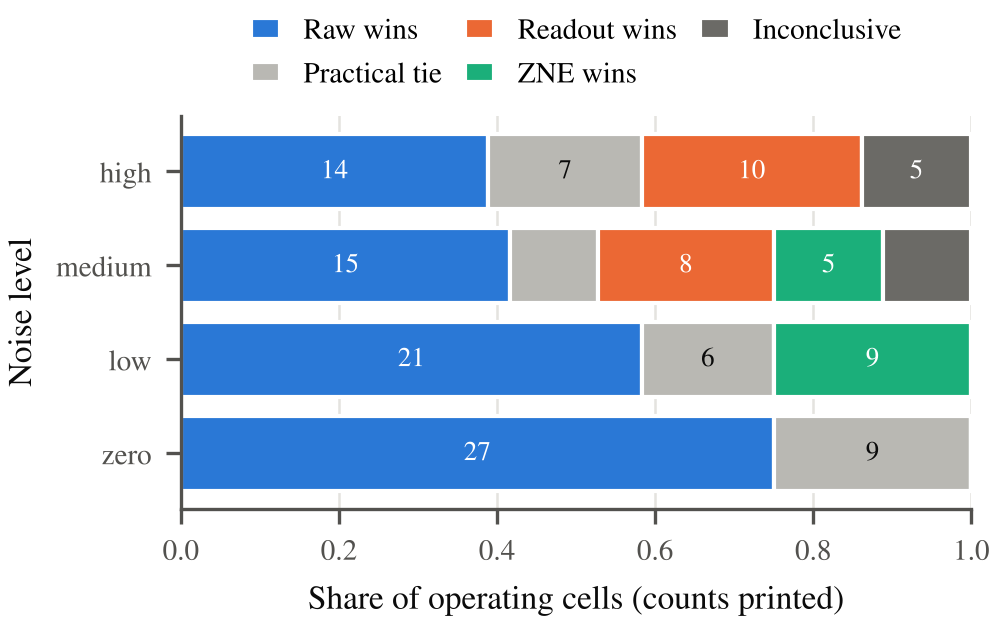
\includegraphics[width=\columnwidth]{fig_regime_shares.png}
\caption{Cost-aware labels by noise level on the main grid. Raw wins most cells at every noise
level; readout and ZNE win in disjoint noise ranges.}
\label{fig:regimes}
\end{figure}

Mitigation can also worsen estimation: \NegativeGains{} of \SummaryRows{} method summaries have
negative RMSE gain relative to raw estimation. Readout produces \HardwareFailures{} explicit
hardware-efficient failures, concentrated at width 6, 1,024 shots, and medium/high noise. These
failures are part of method performance, not missing data.

\subsection{Signal strength and attenuation}
The main grid confounds signal size with circuit family: every boundary-adjacent reference is GHZ
and there is no non-GHZ strong signal. We therefore froze an independent set of 126
hardware-efficient circuits, selected by noiseless value alone into five bands of $|\mu_{\rm ref}|$
from near-zero (below 0.06) to boundary-adjacent (at least 0.9), and ran them under seven noise
conditions at 4,096 and 16,384 shots with 50 repeats.

Figure~\ref{fig:bands} shows the result. Near zero, raw is better in \NearZeroRawBetter{} of
conditions at 4,096 shots; at the boundary, ZNE is better in \BoundaryFitBetter{}. The difference
in ZNE's win share between these bands is \BandContrast{} (interval \BandContrastLow{} to
\BandContrastHigh{}). Raw's wins near zero are not accuracy: its median bias there is 43\% of the
reference. Within bands, ZNE's gain follows the raw attenuation it can remove (Spearman 0.55 to
0.92) more closely than the reference size ($-0.12$ to 0.39). By noise, the linear fit gains 0.020
under depolarizing and amplitude damping and 0.008 under dephasing, but loses 0.006 under coherent
over-rotation, which inverse gates cancel and folding therefore cannot amplify. Global and local
folding gave the same mean gain to three decimals.

\begin{figure}[t]
\centering
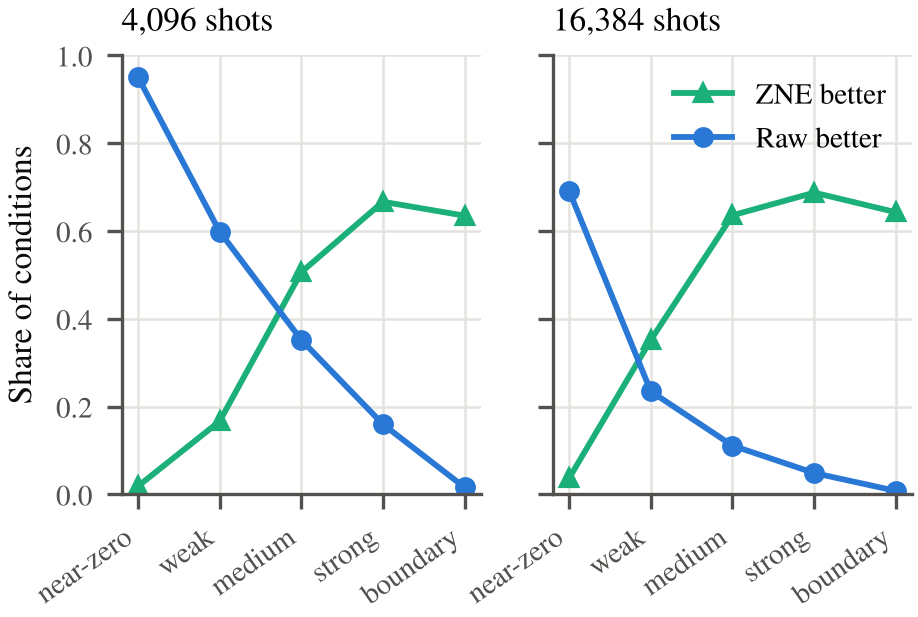
\includegraphics[width=\columnwidth]{fig_signal_bands.png}
\caption{Share of noisy conditions where linear ZNE or raw is better by more than 0.005 in RMSE,
by reference band, on 126 frozen circuits. Raw dominates only where the reference is near zero.}
\label{fig:bands}
\end{figure}

\subsection{Shots to reliability}
Equation~\eqref{eq:decision} predicts that a biased method cannot be rescued by shots. We tested
this on two-candidate decisions sampled from exact channel probabilities, with budgets doubling from
1,024 to $2^{20}$ and 400 repeats. A target is reached at the smallest budget whose Wilson upper
bound, and that of every larger budget, stays at or below it.

Across \ReliabilityCells{} positive-margin cells at a 10\% target, raw reaches it in
\ReachedRaw{}, readout in \ReachedReadout{}, ZNE in \ReachedZne{}, and combined in
\ReachedCombined{}; the rest are blocked by bias (\BlockedRaw{}, \BlockedReadout{}, \BlockedZne{},
and \BlockedCombined{} cells) or not reached by $2^{20}$ shots. Figure~\ref{fig:shots} shows the three
regimes. Without differential bias, raw or readout is cheapest in every cell, and ZNE or combined
needs the same to eight times more shots. With differential readout bias, raw and ZNE error rises
toward one while readout and combined converge. With differential gate-noise bias, only the folding
methods help, and at high noise every method is blocked.

\begin{figure*}[t]
\centering
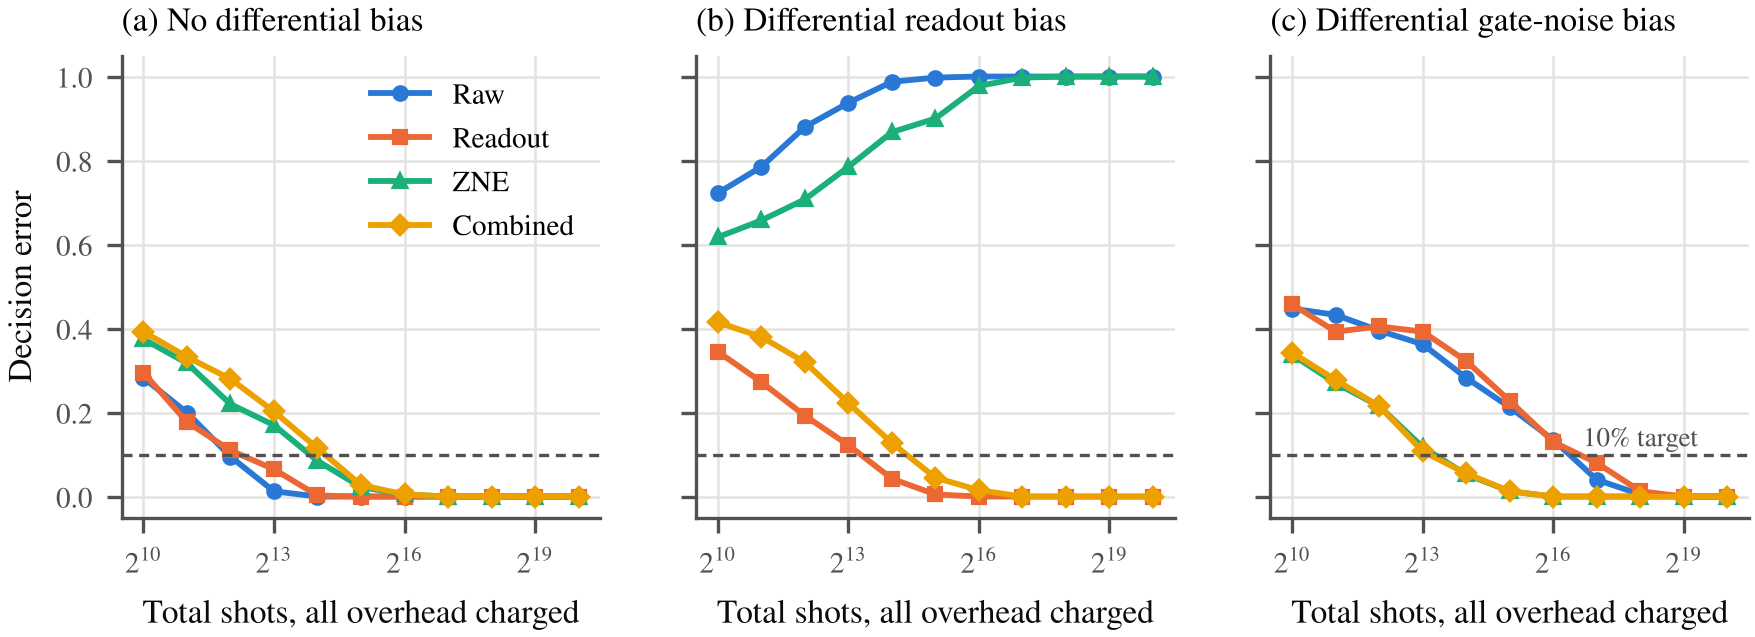
\includegraphics[width=\textwidth]{fig_shots_to_reliability.png}
\caption{Decision error against total budget, all overhead charged, at margin 0.05 (a, b) and 0.10
(c), medium noise, 400 repeats. A method that keeps a differential bias gets worse with more shots.}
\label{fig:shots}
\end{figure*}

\section{Estimator Quality Versus Decision Reliability}
\label{sec:decision}
\subsection{Decision tasks}
Expectation RMSE and decision reliability are distinct. The controlled combined-QEM decision study
shows the separation directly. At margin 0.02, combined decision-error probability ranges from
\CombinedNearTieMinimum{} to \CombinedNearTieMaximum{} across budgets and allocations and does not
consistently beat readout alone. At margin 0.20, nearly all methods resolve the decision. Combined
mitigation has the lowest expectation RMSE in \CombinedExpectationWins{} of
\CombinedExpectationCells{} repository-precommitted conditions, yet all \CombinedValidityRejected{}
of \CombinedValidityCells{} combined-ZNE conditions fail at least one frozen validity criterion, and
\CombinedNegativeInteractions{} of \CombinedInteractionCells{} paired factorial interactions are
negative, so there is no uniform synergy.

\subsection{MaxCut/QAOA candidate selection}
For a graph $G=(V,E)$ and bitstring $z$, the cut value is
$C_G(z)=\sum_{(u,v)\in E}\mathbf{1}[z_u\ne z_v]$. Exhaustive enumeration fixes the optimum for one
width-4 ring, one width-6 sparse graph, and one width-8 medium/dense graph, each with five frozen
$p=1$ QAOA candidates. Each method selects among all five within one budget
$B\in\{4096,16384\}$; the manifest contains 4,500 candidate-level rows and 900 selection groups.

All completed clear-ranking selections identify the ideal best candidate. Near ties separate
estimator quality from decision quality. At 4,096 shots, near-tie error is 0.28 for raw, 0.32 for
readout among completed selections, and 0.36 for ZNE; at 16,384 shots it is 0.17, 0.179, and 0.42.
On the completed 4,096-shot ring and sparse strata, readout lowers energy RMSE from 0.183 to 0.148
and from 0.228 to 0.191, respectively, yet worsens top-1 selection on both; its medium/dense stratum
fails entirely. Across completed repeats, the RMSE--selection-error correlation is only 0.153.

At 16,384 shots, mean regret is 0.0130 for raw, 0.0125 for completed readout selections, and 0.0378
for ZNE. Readout fails all 50 medium/dense selections at 4,096 shots and 22 of 50 at 16,384 shots
because its assignment correction is ill-conditioned; these 72 failed groups are not treated as
abstentions or successes. Results also vary by instance: ZNE's 16,384-shot top-1 error is 0.08 on
the ring, 0.34 on the sparse graph, and 0.50 on the medium/dense graph. Certification is stricter
still: only 2 of 828 completed selections certify a winner under simultaneous intervals. The
remaining 826 completed groups are unresolved.

\subsection{Mechanism: common mode and contrast}
Figure~\ref{fig:mechanism} applies Eq.~\eqref{eq:decomposition}. In panel (a), every arrow from
raw to ZNE points left (lower RMSE) and mostly up (worse selection). Panel (b) shows the medium/dense graph at both budgets. The common-mode term is
small (an RMS of 0.09 against a raw RMSE of 0.81 at 16,384 shots), so energy RMSE is almost entirely
contrast error, and ZNE lowers that contrast error in all six cells. But 77\% of the MSE drop comes
from one low-energy control candidate whose ideal energy (4.72) is far below the leader's (10.22).
Selection depends instead on the gap between the top two candidates: ZNE shrinks its mean from 0.045
to 0.016 and raises its standard deviation from 0.053 to 0.137, and the normal approximation then
predicts inversion rates of 0.20 and 0.45 against the observed 0.18 and 0.50. The share of the MSE
held by non-contenders is specific to this graph (83--86\% against 42--51\% elsewhere), but the
doubling of the gap's spread recurs in every cell (observed ratio 1.92 to 2.58). Off-diagonal error
correlations across repeats are near zero for raw and ZNE, rejecting the hypothesis that raw rankings
are stable because raw errors are shared. Because ZNE's gap standard deviation is
2.09 times raw's at equal shots, ZNE helps selection only if it enlarges the mean contending gap by
more than about 2.09 times. The ring and sparse graphs cannot reach that even with complete
debiasing (at most about 1.33); the medium/dense graph could reach 3.73 but achieves 0.36. This
threshold is derived from the same data and is a hypothesis for new graphs.

\begin{figure*}[t]
\centering
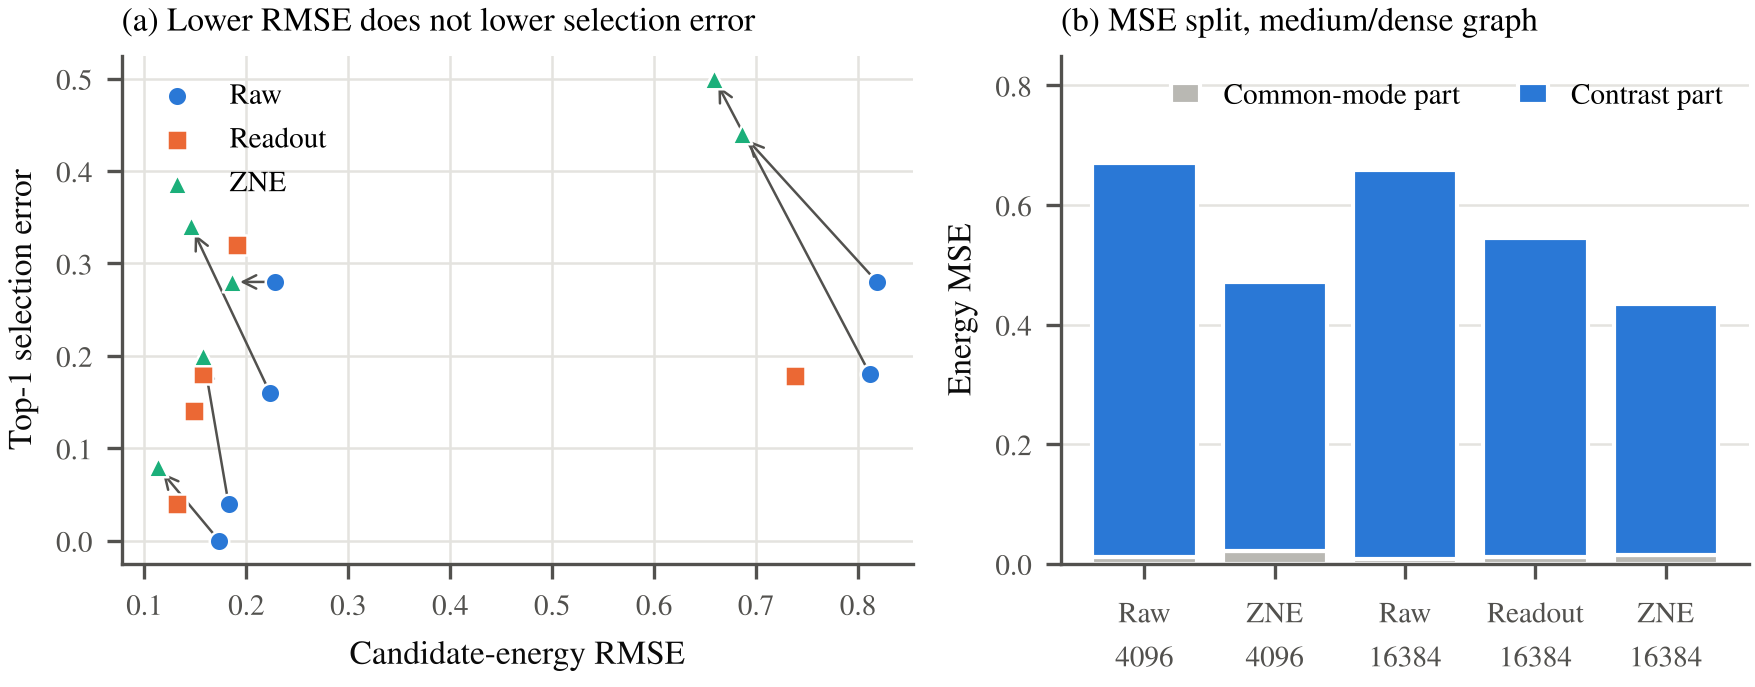
\includegraphics[width=\textwidth]{fig_rmse_vs_selection.png}
\caption{(a) Energy RMSE against top-1 selection error for each QAOA graph, budget, and method;
arrows go from raw to ZNE in the same cell. (b) Energy MSE split into the common-mode and contrast
terms of Eq.~\eqref{eq:decomposition} on the medium/dense graph.}
\label{fig:mechanism}
\end{figure*}

\subsection{Confirmation on new repeats}
The mechanism analysis was exploratory, so we froze a confirmatory plan before collecting new data.
From \ConfirmatoryCount{} committed comparisons, a power analysis on the observed discordant-pair
rate set the repeats each needed for 80\% power against a minimum difference of 0.10 in decision
error or 0.15 in selection error, with Holm correction across the family. Null results are labeled
\emph{close within margin} when the interval lies inside the minimum difference, and
\emph{underpowered} otherwise.

The core counterexample holds: on the medium/dense graph at 16,384 shots, raw errs in
\CoreRawError{} of selections and ZNE in \CoreZneError{} over \CorePairs{} new paired repeats
($p=\CorePValue$). At 4,096 shots the two are within the margin. Overall, \ConfirmResolved{}
comparisons resolve a difference, \ConfirmClose{} are close within the margin, and
\ConfirmUnderpowered{} remain underpowered even at their planned repeats, so the v1-based power
estimates were optimistic for those. On \HoldoutComparisons{} comparisons from two task settings
the original grid never ran, \HoldoutResolved{} resolve, \HoldoutClose{} are close, and
\HoldoutUnderpowered{} are underpowered.

\subsection{Selecting a method adaptively}
\label{sec:selector}
\paragraphlead{Frozen rule selector.}
A non-ML rule selector uses width, depth, declared noise regime, shots, calibration conditioning,
and ZNE fit residuals. On \HoldoutCells{} held-out cells it reaches \HoldoutCompatibilityVTwo{}
decision compatibility. Its diagnostics are 50-repeat cell means that a runtime policy would not
have, so this is an optimistic baseline. Table~\ref{tab:audit} shows what its choices cost.

\begin{table}[t]
\centering
\caption{Consequence audit. Even without charging its diagnostics, the selector has more harmful
outcomes than always-raw across all 180 evaluated cells.}
\label{tab:audit}
\small
\begin{tabular}{lrrrr}
\toprule
Category & Sel. & Raw & Read. & ZNE\\
\midrule
Correct, useful & 63 & 106 & 19 & 18 \\
Correct, tied & 20 & 23 & 11 & 24 \\
Incorrect, negligible & 29 & 0 & 71 & 3 \\
Incorrect, material & 42 & 26 & 45 & 78 \\
Catastrophic & 17 & 16 & 25 & 48 \\
Abstained, avoided failure & 1 & 0 & 0 & 0 \\
Abstained, unnecessary & 5 & 0 & 0 & 0 \\
Inconclusive & 3 & 9 & 9 & 9 \\
\bottomrule

\end{tabular}
\end{table}

Across all cells, the selector has \SelectorHarm{} material or catastrophic outcomes and always-raw
has \AlwaysRawHarm{}. All of raw's harmful outcomes occur in the \StrongSignalCells{} cells with
$|\mu_{\rm ref}|\geq0.06$, so raw is not a general policy either.

Among diagnostics, condition number acts only as a warning: readout is reliable in 75\% of
cells below 1.5, 50\% from 1.5 to 3, 10\% from 3 to 8, and none of the 4 cells at 8 or above.
ZNE fit residual does not discriminate, with rates of 24--33\% in every adequately sampled bin.
Three cells flip across the condition-number gate of 8 under repeat resampling, with means of
7.87, 8.10, and 8.16. Table~\ref{tab:envelope} lists every single-feature level supported for
reliable use; none exists for ZNE, and the frozen joint envelope is empty.

\begin{table}[t]
\centering
\caption{Single-feature levels supported for reliable use. None exists for ZNE.}
\label{tab:envelope}
\small
\begin{tabular}{llrr}
\toprule
Method & Level & Reliable & Stable\\
\midrule
Raw & width 6 & 36/44 & 55\% \\
Raw & noise zero & 32/32 & 100\% \\
Raw & $|\mathrm{ref}|$ $<0.06$ & 56/56 & 100\% \\
Raw & margin 0.2 & 11/12 & 93\% \\
Readout & noise zero & 29/32 & 89\% \\
Readout & $|\mathrm{ref}|$ $\geq$ 0.5 & 26/30 & 88\% \\
Readout & margin 0.2 & 11/12 & 94\% \\
\bottomrule

\end{tabular}
\end{table}

\paragraphlead{Repository-precommitted selector test.}
A runtime selector sees only one repeat's pilot, which spends 25\% of the budget. The selector test
uses a fresh grid committed before it ran, with \VTwoCells{} cells and 24,000 rows. All three frozen
criteria fail, so the runtime selector is a no-go. For H1, \VTwoReliableCells{} of
\VTwoDecidedCells{} decided cells are reliable (lower bound \VTwoHOneLow{}). For H2,
\VTwoAvoidedCells{} of \VTwoNoSafeCells{} no-safe cells avoid a failure (lower bound
\VTwoHTwoLow{}). For H3, mean regret on decided cells is \VTwoRegretSelector{}, against
\VTwoRegretRaw{} for always-raw and \VTwoRegretReadout{} for always-readout. As an exploratory
reading, raw is reliable in all 36 cells with $|\mu_{\rm ref}|<0.06$ and readout in 34 of 48 with
$|\mu_{\rm ref}|\geq0.5$, but a runtime policy does not know the reference.

\paragraphlead{Selector with abstention (v3).}
The third selector chooses the largest of three candidate values. It spends 10\% of the budget on
calibration and 20\% on a pilot at folds 1, 3, 5, defaults to readout correction, switches to combined
mitigation only when both pilot contenders show a resolved rise in magnitude after extrapolation,
may fall back to raw when correction is unresolved on every candidate, and abstains when its two
calibrations disagree or the final top gap is unresolved. The rule was chosen from a 30-rule grid
on training and validation tasks drawn from four circuit families (hardware-efficient, rotated GHZ,
transverse-field Ising Trotter steps, and ring QAOA; 72 tasks in total) and scored once on 20
held-out tasks. Table~\ref{tab:selector3} shows the result: forced regret
\ThreeRegretSelector{} against \ReadoutThreeRegret{} for always-readout, at \ThreeCostRatioSelector{}
times the two-qubit gate executions, and lower reliable coverage than the same abstention rule
applied to readout alone. No frozen acceptance route passed, so adaptive selection did not beat a
simple fixed strategy. Always-raw had the lowest regret in every holdout group: the candidates share
one readout, so its bias is common-mode and cancels in the comparison.

\begin{table}[t]
\centering
\caption{Held-out selector comparison, 20 tasks and 14,000 runs. Reliable coverage is the share of
runs that are covered and correct. The oracle picks the best baseline per condition after scoring.}
\label{tab:selector3}
\footnotesize
\setlength{\tabcolsep}{3pt}
\begin{tabular}{@{}lrrrr@{}}
\toprule
Policy & Coverage & Regret & Reliable & Gate shots\\
\midrule
Always raw & 1.00 & 0.0024 & 0.919 & 113,664\\
Always readout & 1.00 & 0.0031 & 0.908 & 90,931\\
Always ZNE & 1.00 & 0.0059 & 0.867 & 340,992\\
Always combined & 1.00 & 0.0072 & 0.855 & 272,794\\
Selector (v3) & 0.64 & 0.0031 & 0.630 & 147,767\\
Abstaining readout & 0.68 & 0.0033 & 0.666 & 147,763\\
Oracle baseline & 1.00 & 0.0022 & -- & --\\
\bottomrule
\end{tabular}
\end{table}

\section{Validity and Operational Boundaries}
\label{sec:boundaries}
\subsection{ZNE validity gates}
An extrapolate is not credible merely because it moves toward the reference. The first gate
requires retained signal, physical bounds, positive gain with uncertainty, an advantage over
matched-cost garbage folding, and few destroyed or unstable repeats. It accepts only
\ZNECredibleCells{} of \ZNEValidityCells{} simulated cells, all Bell-state conditions, and none of
the \ZNEHardwareCells{} hardware-efficient cells, matching concerns about artefactual ZNE
improvement \cite{koster2026}. A post hoc audit found two weaknesses: two of its checks read the
exact reference, and its trend check partly double counts physical-bound violations.

We therefore chose a runtime-only gate from 256 candidates (four physical-bound variants, eight
trend variants, and optional garbage, retention, and estimated-gain checks) on training and
validation circuits of the frozen signal set, and scored it once on 30 held-out circuits. ``Really
improved'' means the fit's RMSE, from independent draws, beats raw by more than 0.005. The frozen
choice reduced to a single slope-sign stability check. Figure~\ref{fig:gate} shows the holdout:
false acceptance \GateVTwoFA{} and false rejection \GateVTwoFR{}, against \GateVOneRuntimeFA{} and
\GateVOneRuntimeFR{} for the runtime checks of the first gate and \GateVOneFullFA{} and
\GateVOneFullFR{} for the full first gate, which reads the exact value. Every one of the 230 holdout
rejections names its failure mechanism. The selected check measures whether the decay across
folds is resolved, not whether the extrapolate is right, so its false acceptance rises with shots
(0.131 at 4,096, 0.224 at 16,384) and reaches 0.414 under amplitude damping. Leave-one-factor-out,
weighted-residual, and quadratic-agreement checks scored below chance, and the model
selection rule (local folding with an exponential fit) did not beat the default linear fit on
holdout.

\begin{figure}[t]
\centering
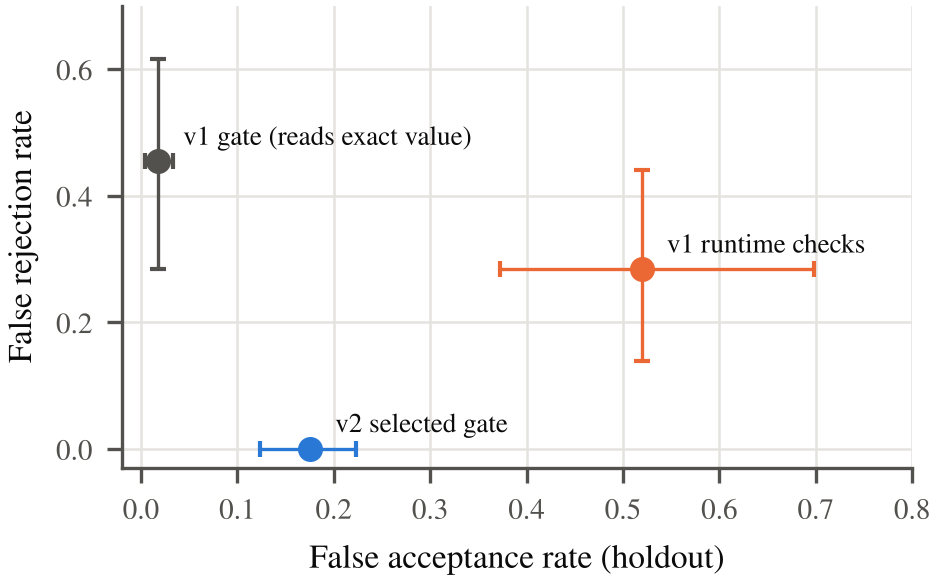
\includegraphics[width=\columnwidth]{fig_zne_gate_holdout.png}
\caption{Holdout error rates of three ZNE gates on 30 circuits not used to choose them. Bars are
circuit-cluster bootstrap intervals; the v2 gate had no false rejection in any resample.}
\label{fig:gate}
\end{figure}

\subsection{Certification}
\paragraphlead{Sequential stopping.}
Two candidates are sampled in batches until an interval for their gap excludes zero; every look is
tested at $\alpha/K$. At margin 0, where any certification is false, Wilson stopping certifies in
\NullWilsonMin{}--\NullWilsonMax{} of repeats, whereas uncorrected peeking reaches
\NullNaiveMin{}--\NullNaiveMax{}. Table~\ref{tab:sequential} shows the trade-off: stopping early
saves shots but leaves more decisions unresolved. Certification does not detect bias: with strong
gate-noise imbalance at margin 0.05, raw certifies the wrong candidate in \BiasedRawWrong{} of
repeats after a mean of \BiasedRawShots{} shots, and ZNE still does so in \BiasedZNEWrong{}.

\begin{table}[t]
\centering
\caption{Stopping early saves shots but leaves more symmetric-task decisions unresolved
(16,384 shots, margins above 0, nonzero noise).}
\label{tab:sequential}
\small
\begin{tabular}{llrrr}
\toprule
Method & Policy & Shots & Unres. & Wrong\\
\midrule
Raw & Fixed budget & 16{,}384 & 27.1\% & 0.08\% \\
Raw & Wilson & 9{,}583 & 40.7\% & 0.00\% \\
Raw & Gap confidence & 10{,}653 & 48.2\% & 0.00\% \\
Raw & Variance aware & 14{,}136 & 70.8\% & 0.00\% \\
Raw & Naive peeking & 5{,}067 & 16.2\% & 3.25\% \\
Readout & Wilson & 11{,}429 & 43.7\% & 0.08\% \\
ZNE & Wilson & 13{,}045 & 63.6\% & 0.08\% \\
\bottomrule

\end{tabular}
\end{table}

\paragraphlead{Two-layer certification.}
On the 20 held-out selector tasks, five independent batches each carry their own calibration.
Layer 1 requires the winner to beat every challenger by a one-sided $t$ test on batch differences,
which keeps shared calibration within a batch rather than assuming independence. Layer 2 requires
six bias alarms to stay silent: raw and corrected winners differing, a reversal of the gap at fold 5,
calibration drift between batches, an out-of-bound value, variance amplification, and batch sign
instability. Both layers certify \BothLayersCertified{} of runs with false certification
\BothLayersFalse{} per run; Layer 1 alone certifies \LayerOneCertified{}; a naive test that treats
all estimates as independent certifies \NaiveCertified{} with \NaiveFalse{} false certifications
per run. Figure~\ref{fig:certification} shows where the errors are. The alarms fired in at most
2.4\% of Layer-1 passes, so the second layer barely changed anything. Near-tie tasks fail:
\CertWrongNearTie{} of certified runs pick the wrong winner, because the bias survives every layer.
Coherent over-rotation has the highest false certification of any noise, \CertWrongOverrotation{}
of certified runs.

\begin{figure}[t]
\centering
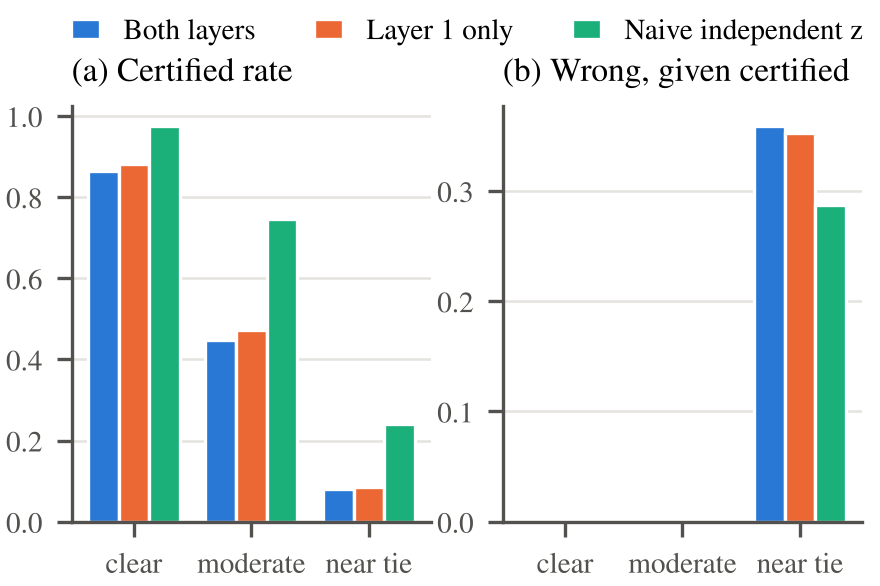
\includegraphics[width=\columnwidth]{fig_certification.png}
\caption{Certification on 20 held-out tasks by ideal gap class. Correcting for shared samples
(blue, orange) lowers false certification on clear and moderate tasks, but no rule controls it on
near ties.}
\label{fig:certification}
\end{figure}

\subsection{Readout correction at scale}
Under one shared budget, full-matrix correction gives each of $2^w$ calibration states very few
shots: 3 at width 8 and 4,096 shots. It is ill-conditioned or singular in \FullFailLow{} to
\FullFailHigh{} of width-8 runs at 4,096 shots and fails always at width 10
(Fig.~\ref{fig:readout}). At 16,384 shots it completes at width 8 but is worse than no correction.
Given 1,024 shots per calibration circuit instead, it completes at widths 8 and 10 using
\FullQualityShareLow{} to \FullQualityShareHigh{} of all shots for calibration. Full-matrix failure is
therefore a resource failure, not a method failure. The model matters more than the budget:
under pair-correlated readout, tensor-product, observed-subspace, and matrix-free correction all
assume independent errors and become worse than no correction, while pairwise-local correction
stays below 0.05 at every width. Observed-subspace and matrix-free solvers match tensor-product
correction wherever it is correct.

\begin{figure*}[t]
\centering
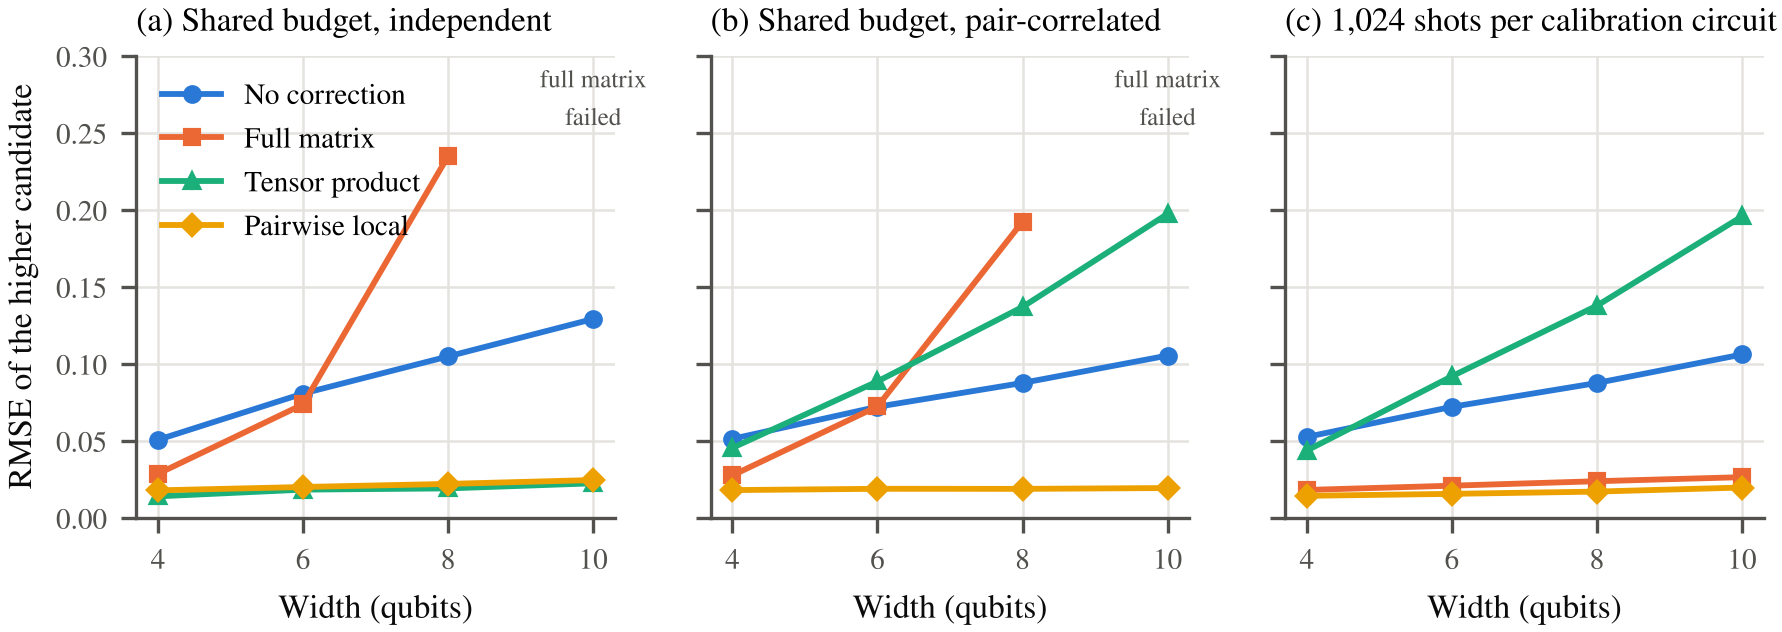
\includegraphics[width=\textwidth]{fig_readout_width.png}
\caption{RMSE of a parity observable on qubits 0 to $w-2$ against width, 200 repeats. Under a shared
budget, full-matrix correction fails by width 8 to 10; with correlated readout, an independent model
does worse than no correction.}
\label{fig:readout}
\end{figure*}

\subsection{Calibration mismatch and early warning}
We calibrated once on $A_{\rm cal}$ and measured under
$A_{\rm eval}(\lambda)=(1-\lambda)A_{\rm cal}+\lambda A_{\rm mis}$ for 21 values of $\lambda$.
Mitigation lost to raw only under asymmetric drift (from $\lambda=0.25$ to 0.60, later at larger
width) and under a change from independent to fully pair-correlated flips with equal marginals
(from 0.50 to 0.75; Fig.~\ref{fig:mismatch}). Under abrupt change, calibration age, and added pair
flips it stayed better than raw up to $\lambda=1$, because raw suffers the same errors. As
predicted, the calibration condition number never warned (\ConditionWarnShare{} of cases), since it
comes from the stale calibration. A 1,024-shot check of the two basis states warned in time in
\CheckWarnShare{} of cases, but it is blind to the change to correlated flips, because the
marginals it measures do not change, and that is one of the two scenarios where mitigation loses.
Decision error never rose steeply at margin 0.10, so that question is unanswered by this design.

\begin{figure*}[t]
\centering
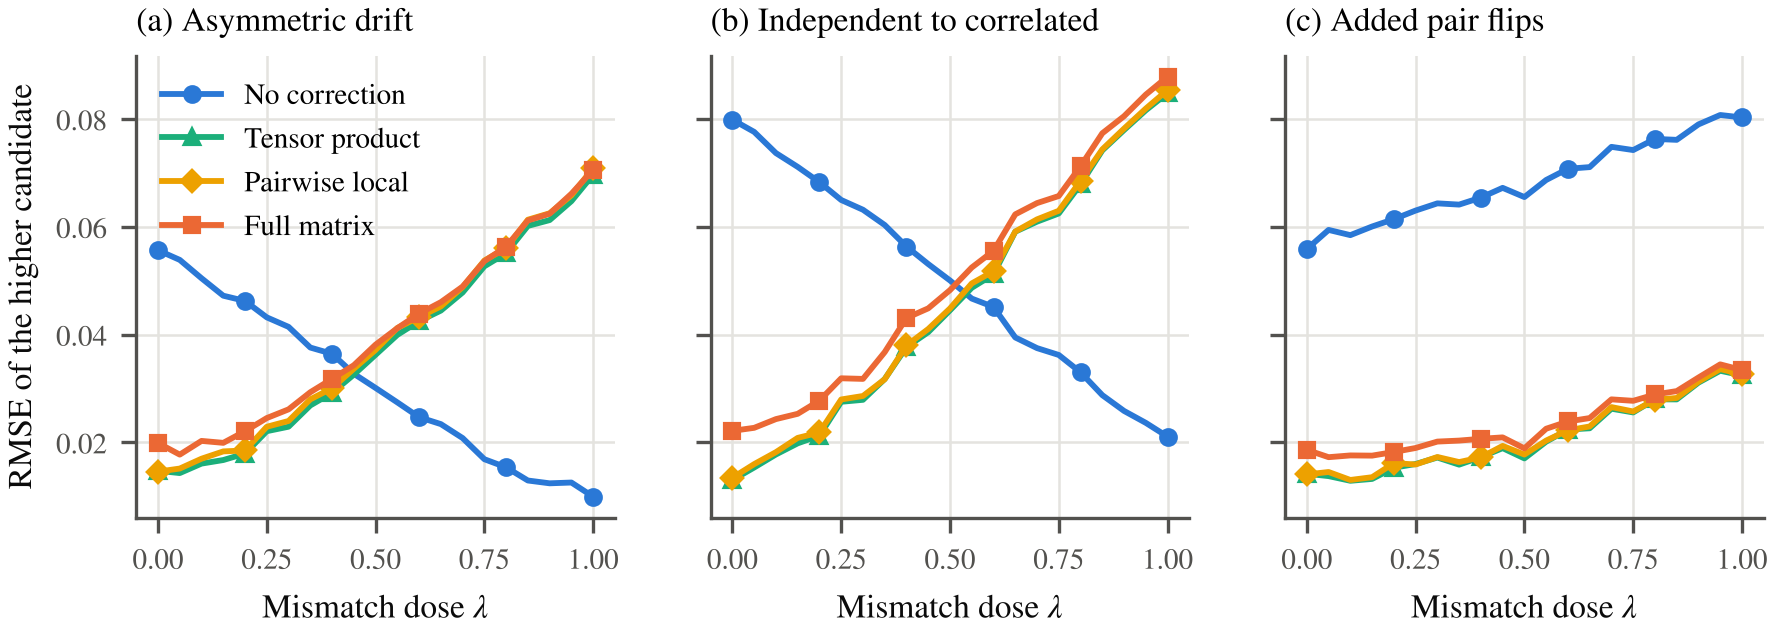
\includegraphics[width=\textwidth]{fig_mismatch_dose.png}
\caption{Readout mismatch dose-response at width 6, 150 repeats. Corrections lose to raw under
asymmetric drift (a) and a change to correlated flips (b), but not under added pair flips (c).}
\label{fig:mismatch}
\end{figure*}

\subsection{Calibration reuse under drift}
Table~\ref{tab:lifetime} compares policies over 100 decisions in the first drift study. Triggered
recalibration has decision error close to recalibrating every time at about \TriggerShotSaving{}
lower cost, while never recalibrating fails under directed drift. A larger sweep over drift
amplitude, timescale, shape, run length, margin, calibration cost, and trigger threshold, with all
check shots charged, gives the same picture (Fig.~\ref{fig:drift}). A trigger at $z=2$ matches or beats
every-decision recalibration in mean decision error with about 60\% of the shots, except under
sinusoidal drift at amplitude 0.06; stricter triggers lose there. Every-decision recalibration
also adds fresh calibration noise at each step.

\begin{table}[t]
\centering
\caption{A triggered policy approaches every-decision reliability at lower cost (first drift
study, 100 decisions).}
\label{tab:lifetime}
\small
\begin{tabular}{lrr}
\toprule
Recalibration & Shots per decision & Error\\
\midrule
Every decision & 2{,}048 & 0.062 \\
Every 10 decisions & 1{,}126 & 0.074 \\
Uncertainty trigger & 1{,}229 & 0.067 \\
Never & 1{,}034 & 0.234 \\
\bottomrule

\end{tabular}
\end{table}

\begin{figure}[t]
\centering
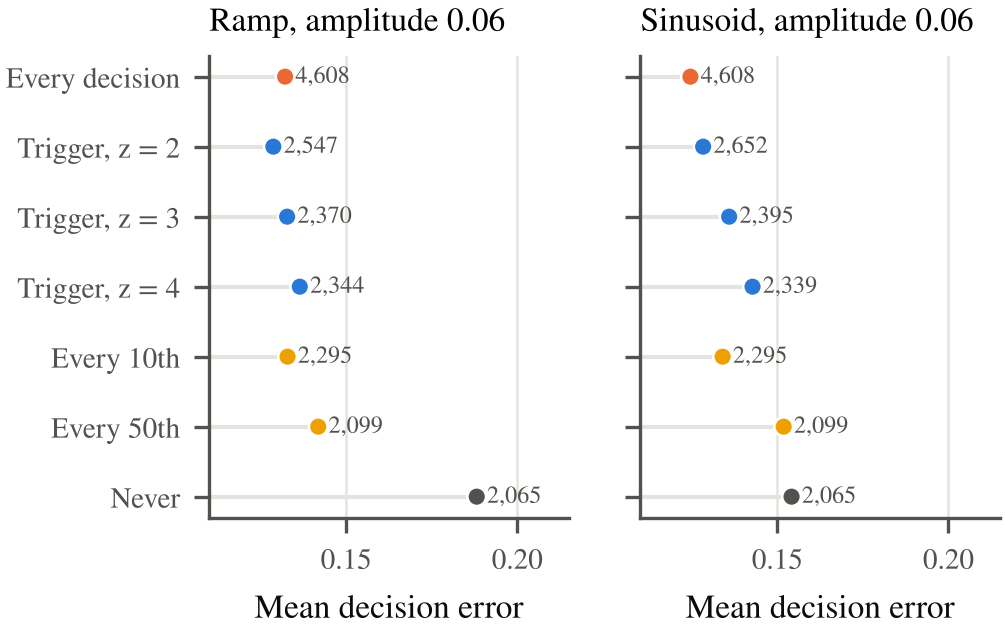
\includegraphics[width=\columnwidth]{fig_drift_policy.png}
\caption{Recalibration policies under drift of amplitude 0.06, averaged over the other sweep
parameters. Labels give total shots per decision, including calibration and check circuits.}
\label{fig:drift}
\end{figure}

\subsection{Hardware readiness}
Table~\ref{tab:hardware} lists frozen predictions for six candidate device cells. The review decision
is no-go: only \HardwareGoMet{} of \HardwareGoTotal{} go requirements is fully met, and all
\HardwareTriggers{} no-go triggers apply. The plan would need about \HardwareTotalShots{} million
shots. The positive control is credible at 16,384 shots but rejected at 4,096, three of five
ZNE-relevant cells have no single-method validity assessment, and no code captures device
metadata. This is a measured outcome of the review, not a statement about how any device would
behave, since no job was submitted.

\begin{table}[t]
\centering
\caption{Frozen simulator predictions for proposed device cells at 16,384 shots, or a 100-decision
workload for calibration reuse. These are hypotheses for a device, not hardware results. Val.\ is
single-method ZNE validity; Mshots is the planned total in millions.}
\label{tab:hardware}
\footnotesize
\setlength{\tabcolsep}{2.4pt}
\begin{tabular}{lrrrrlr}
\toprule
Cell & Raw & RO & ZNE & Comb. & Val. & Mshots\\
\midrule
Readout-dominated & 0.740 & 0.893 & 0.791 & 0.958 & credible & 3.3 \\
ZNE control & 0.970 & 0.987 & 0.980 & 0.997 & credible & 4.1 \\
ZNE signal risk & 0.232 & 0.263 & 0.265 & 0.305 & none & 4.1 \\
Near tie & 0.012 & 0.021 & 0.014 & 0.021 & none & 41.0 \\
Clear margin & 0.179 & 0.181 & 0.184 & 0.188 & none & 3.3 \\
Calibration reuse & 0.510 & 0.530 & -- & -- & -- & 16.3 \\
\bottomrule

\end{tabular}
\end{table}

\section{Negative Results by Mechanism}
\label{sec:negative}
Table~\ref{tab:negative} classifies each negative or inconclusive result. A \emph{method} failure
persists with unlimited shots; a \emph{resource} failure disappears with more calibration or target
shots; a \emph{model} failure comes from a wrong noise or readout model.

\begin{table*}[t]
\centering
\caption{Negative and inconclusive results. ``Driven by'' is deterministic (D) or sampling (S); ``More
shots'' says whether a larger budget removes the failure; ``Runtime signal'' names a diagnostic that
predicted it, if any. These are review judgments based on the reported data.}
\label{tab:negative}
\footnotesize
\setlength{\tabcolsep}{4pt}
\begin{tabular}{@{}p{0.27\textwidth}lp{0.08\textwidth}p{0.15\textwidth}p{0.17\textwidth}p{0.18\textwidth}@{}}
\toprule
Result & Driven by & Type & More shots & Runtime signal & Reproduced across\\
\midrule
Raw beats mitigation in most main-grid cells & D & Resource & No (cost is structural) & Small $|\widehat\mu|$ & Grid, signal set, selector tasks\\
Lower RMSE, worse QAOA selection & D + S & Method & No (variance factor 4.375) & None found & 3 graphs; confirmed at 16,384\\
Biased method misses a decision target & D & Method & No; error rises & None & 3 task types\\
ZNE gate false acceptance & D & Method & No; rises with shots & Slope check is the gate & Holdout, all noises\\
Model-selection rule underperforms & S & Statistical & Possibly & -- & One holdout\\
Adaptive selectors (v1, v2, v3) & D + S & Resource & Unknown & -- & Three designs\\
Near-tie false certification & D & Method & No & None & All noises\\
Bias alarms rarely fire & D & Method & No & -- & One holdout\\
Full matrix fails at width 8 & D & Resource & Yes, at 80--98.5\% calibration share & Condition number & Widths 8, 10; 3 models\\
Independent model under correlated readout & D & Model & No & Pairwise calibration & Widths 4--10\\
Check circuit blind to correlation change & D & Model & No & -- & Widths 4--8\\
No steep decision-error rise found & -- & Design & -- & -- & Inconclusive\\
\bottomrule
\end{tabular}
\end{table*}

\section{Verification and Reproducibility}
\label{sec:verification}
Raw repeat-level rows are never replaced by summaries. \texttt{src.verify\_final\_project}
recomputes the main summaries from raw rows at tolerance $10^{-9}$, accounts for every manifest, and
checks figures and this document. \texttt{src.claim\_ledger} separately checks 22 computed claims
covering 189 printed numbers without importing project code, and labels computed results, manual
interpretation, hypotheses, limitations, and review judgments. Of these claims, 11 are recomputed from
raw repeat rows, 8 from processed tables (for example, the signal study's truth table, whose fit
errors agree with normal theory to within 0.0014), 2 from manifests, and 1 from a processed table
only. Every number generated for Sections~\ref{sec:budget} to~\ref{sec:boundaries} is recomputed
except one ratio of gate executions, which needs the project's circuit builders. Five
deterministic sampled claims are recomputed from repeat rows after a correction to the audit
implementation. Eight tables and the figures have source provenance but have not all been
independently recomputed, so the paper as a whole is not independently verified.
Replacing the original BCa interval with a deterministic percentile-bootstrap sensitivity
calculation did not change the 144 cell labels.

An artifact registry declares every generator, its configs, manifests, outputs, and expected rows,
and \texttt{src.artifact\_provenance} records a content hash for every tracked artifact.
Continuous integration rebuilds every routine generator from a clean clone on each push. The 16
long generators of the release scope are rebuilt by a separate workflow, one job per generator, each
deleting that generator's committed outputs in a clean clone, running it with the locked
dependencies, and comparing the result with the committed files. When this version was written,
that workflow had not yet completed, so the largest raw files had not been regenerated in a clean
environment. NumPy's binomial stream changes between versions, so a rebuild with another NumPy
version should be expected to differ slightly in sampled rows.

\texttt{src.independent\_reference} reproduces exact values within $10^{-12}$ and, from fixed
counts, all completed QAOA selections. It does not check noisy sampling. Width-8 readout energies
differ by up to about $10^{-6}$. The later studies use a density-matrix simulator checked against
Aer. Both implementations were written by the same author.

\section{Discussion}
\paragraphlead{What the evidence supports.}
The strongest conclusions are structural rather than empirical accidents. Equal accounting reverses
rankings whenever no decision-relevant bias exists, because calibration and folding cost shots that
raw estimation spends on the target. Bias cannot be bought off with shots, and every
interval-based tool we tested, from sequential stopping to two-layer certification, controls only
sampling error. Runtime diagnostics see changes in marginals and resolved decays, not hidden bias or
a change in correlation structure. And a correctly modeled local correction succeeds where a
mismodeled one does worse than nothing.

\paragraphlead{Rule freezing and independence.}
The combined, QAOA, scalable-readout, runtime-selector, signal, gate, confirmatory, selector-v3, and
readout-boundary protocols were committed before their result artifacts. The first ZNE gate's checks
were named in advance, but its numerical thresholds and results first appeared together in the same
repository state; therefore this is not an independently timestamped preregistration. The
sequential and calibration studies and the first selector use frozen repository rules that first
appear with their results. Commit order proves repository publication order only, not the
wall-clock order of design or execution. In the readout-boundary study, a 20-repeat smoke run showed
that an all-qubit parity is blind to pair flips; the observable was changed before freezing, and no
hypothesis, threshold, or grid value changed.

\paragraphlead{Limitations.}
All noisy values are simulator-derived with synthetic noise; there is no device drift, calibrated
crosstalk, leakage, or non-Markovian noise. The main grid has one hardware-efficient circuit per
width and depth, so width and depth effects are confounded with specific angles. The QAOA study has
three curated graphs with $p=1$; its candidates are frozen inputs whose exact-tie ordering depends on
the generating machine. The signal and selector holdouts have 30 circuits and 20 tasks, and
candidates in the selector tasks share one readout, which favors raw estimation. The scalable-readout
manifest planned 960 repeats of correlated readout at widths 8--12 that were never run; correlated
models ran only at widths 2--6 in the original mismatch study and in the separate readout-boundary
protocol, whose rows are not merged into the original table. The drift sweep uses one qubit.

\paragraphlead{Why the hardware review ends in no-go.}
A disagreement between a device and Table~\ref{tab:hardware} would first falsify the transfer of a
synthetic noise model, not the simulated conclusion. Separating drift from method failure needs
interleaved circuits, repeated reference controls, and a calibration record around each block, none
of which exists here. A run now would mainly produce a demonstration, so a no-go is the more honest
result. The cheapest informative device question is whether real readout carries enough pair
correlation to make independent models worse than none, which needs calibration circuits only.

\section{Conclusion}
No QEM method is uniformly useful under fixed-budget accounting, and better estimation is not
better decision-making. Mitigation pays off when it removes a bias that differs between the
alternatives being compared and that is larger than its own variance cost; it does not pay off
when the error is common-mode, when the method's model is wrong, or when its calibration consumes the
budget. Adaptive selection, statistical certification, and the diagnostics we tested could not
identify these cases reliably at runtime, so simple fixed policies remain the reference that any
adaptive rule must beat, and bias detection is the central open problem.

\bibliographystyle{abbrv}
\bibliography{references}

\appendix
\section{Reproducibility}
{\footnotesize
\begin{verbatim}
python -m pytest
python -m src.verify_generated_artifacts
python -m src.verify_generated_artifacts \
    --scope release --module src.generate_signal_v2
python -m src.generate_signal_v2 --workers 2
python -m src.zne_gate_v2
python -m src.confirmatory_v1
python -m src.confirmatory_qaoa_v1
python -m src.shots_to_reliability
python -m src.generate_selector_v3 --workers 4
python -m src.generate_readout_feasibility_v2 --workers 4
python -m src.generate_readout_mismatch_dose --workers 4
python -m src.generate_drift_policy --workers 4
python -m src.generate_paper_v2_assets
python -m src.artifact_provenance --write
python -m src.verify_final_project
python -m src.claim_ledger
\end{verbatim}
}
The full release scope runs as one job per generator in
\texttt{.github/workflows/rebuild-generators.yml}. Protocols are in \texttt{docs/}: \texttt{signal\_v2\_protocol.md}, \texttt{parts\_7\_8\_protocol.md},
and \texttt{part\_9\_protocol.md}, with results in \texttt{signal\_v2\_results.md} and
\texttt{parts\_7\_9\_results.md}.

\section{Gate definitions}
The first ZNE gate passes a cell when the lower 95\% bound of final-fold retention exceeds 0.10, the
physical overshoot is at most $10^{-12}$, signed-probability negative mass is at most 0.05, the
lower bounds of the garbage-control advantage and of the paired gain exceed zero, no repeat is signal
destroyed, and at most 5\% are unstable. The second gate's candidates and selection rule, the
selector grid, and the certification alarms are listed in the protocol files above, with every
threshold fixed before the corresponding run.

\section{Evidence by track}
Table~\ref{tab:evidence} separates each original finding by evidence type. The hardware column is
empty for every track.

\begin{table*}[t]
\centering
\caption{Evidence matrix for the original tracks. Y marks evidence of that type; An.\ is analytic,
NL noiseless simulation, NS noisy simulation, HW hardware.}
\label{tab:evidence}
\footnotesize
\begin{tabular}{@{}p{0.10\textwidth}@{\hspace{4pt}}c@{\hspace{3pt}}c@{\hspace{3pt}}c@{\hspace{3pt}}c@{\hspace{5pt}}p{0.325\textwidth}p{0.195\textwidth}p{0.195\textwidth}@{}}
\toprule
Track & An. & NL & NS & HW & Supported finding & Unresolved question & Limitation\\
\midrule
Expectation accuracy & Y & Y & Y & -- & No universal winner: 77 raw, 26 ties, 18 readout, 14 ZNE. & Which method wins when the signal is strong and the circuit is new? & Raw wins are mostly near-zero references; one circuit per width and depth. \\
Decision reliability & Y & Y & Y & -- & Lower RMSE does not ensure a better decision; near-tie error is 0.26-0.48 for combined QEM. & How does this extend beyond two candidates? & Controlled margins on small circuits. \\
ZNE validity & Y & Y & Y & -- & Apparent gain is not validated gain: 5 of 16 cells pass, none hardware-efficient. & Does the gate hold for other circuits and fits? & Two circuits, linear fit, and folds 1, 3, and 5. \\
Combined mitigation & -- & Y & Y & -- & Lowest RMSE in 12 of 16 conditions, yet all 16 validity checks fail. & Are readout and gate errors separable on a device? & Six cells, two budgets, two allocations, higher overhead. \\
Readout scalability & Y & Y & Y & -- & Lower memory is not robustness: mismatch error reaches 0.88-0.94. & How large is real correlated readout error? & Synthetic channels; correction amplifies sampling spread. \\
Application case study & Y & Y & Y & -- & Lower energy RMSE does not imply better selection; 2 of 828 completed selections certify. & Does this hold for other graphs and depths? & Three graphs, five frozen candidates, and p=1. \\
Calibration drift & -- & -- & Y & -- & Triggered recalibration saves about 40\% of shots with similar error; never recalibrating reaches 0.386 under abrupt drift. & What drift does a real device show? & Directed synthetic stress; not a physical lifetime. \\
Sequential certification & Y & Y & Y & -- & Corrected looks keep false certification at or below 2.7\%, versus up to 24.9\% for peeking; bias is not detected. & How can bias be detected before certifying? & Two-qubit circuits, one observable, conservative bounds. \\
Hardware readiness & -- & -- & Y & -- & Review decision: no-go. No job was submitted. & Can a backend-specific, powered, controlled protocol be justified? & Predictions depend on simulator noise; no backend data. \\
\bottomrule

\end{tabular}
\end{table*}
\end{document}
